\section{Ainul Filiani}
\subsection{Praktek}
\subsubsection{Buatlah fungsi (file terpisah/library dengan nama NPM realtime.py) untuk mendapatkan data langsung dari arduino}
\lstinputlisting[firstline=8, lastline=14]{src/5/1174073/praktek/1174073_realtime.py}

\subsubsection{Buatlah fungsi (file terpisah/library dengan nama NPM save.py) untuk mendapatkan data langsung dari arduino dengan looping}
\lstinputlisting[firstline=8, lastline=15]{src/5/1174073/praktek/1174073_save.py}

\subsubsection{Buatlah fungsi (file terpisah/library dengan nama NPM realtime.py) untuk mendapatkan data dari arduino dan langsung ditulis kedalam file csv}
\lstinputlisting[firstline=16, lastline=29]{src/5/1174073/praktek/1174073_realtime.py}

\subsubsection{Buatlah fungsi (file terpisah/library dengan nama NPM csv.py) untuk membaca file csv hasil arduino dan mengembalikan ke fungsi}
\lstinputlisting[firstline=9, lastline=17]{src/5/1174073/praktek/1174073_csv.py}

\subsubsection{Penanganan Error}
Untuk kali ini saya menemukan Type Error, yaitu error yang menampilkan jika type data na berbeda berusaha disatukan.
\lstinputlisting[firstline=8, lastline=18]{src/5/1174073/praktek/1174073.py}
%%%%%%%%%%%%%%%%%%%%%%%%%%%%%%%%%%%%%%%%%%%%%%%%%%%%%%%%%%%%%%%%%%%%%%%%%%%%%%%%%%%%%

\section{Alfadian Owen}
\subsection{Soal 1}
Buatlah fungsi untuk mendapatkan data langsung dari arduino
\lstinputlisting[firstline=7, lastline=14]{src/5/1174091/Praktek/1174091_realtime.py}

\subsection{Soal 2}
Buatlah fungsi untuk mendapatkan data langsung dari arduino dengan looping
\lstinputlisting[firstline=7, lastline=15]{src/5/1174091/Praktek/1174091_save.py}

\subsection{soal 3}
Buatlah fungsi untuk mendapatkan data dari arduino dan langsung ditulis kedalam file csv
\lstinputlisting[firstline=16, lastline=25]{src/5/1174091/Praktek/1174091_realtime.py}

\subsection{Soal 4}
Buatlah fungsi untuk membaca file csv hasil arduino dan mengembalikan ke fungsi
\lstinputlisting[firstline=7, lastline=15]{src/5/1174091/Praktek/1174091_csv.py}

\subsection{Penanganan Error}
Buatlah fungsi untuk membaca file csv hasil arduino dan mengembalikan ke fungsi
\lstinputlisting[firstline=7, lastline=15]{src/5/1174091/Praktek/1174091_error.py}

%%%%%%%%%%%%%%%%%%%%%%%%%%%%%%%%%%%%%%%%%%%%%%%%%%%%%%%%%%%%%%%%%%%%%%%%%%%%%%%%%%%%%%%%%%%%%%%
\section{Alvan Alvanzah/1174077}
\subsection{Ketrampilan Pemrograman}
\begin{enumerate}
    \item Buatlah  fungsi  (file  terpisah/library  dengan  nama  NPMrealtime.py)  untuk mendapatkan data langsung dari arduino.
    \lstinputlisting[firstline=1, lastline=7]{src/5/1174077/praktek/1174077_realtime.py}
    
    \item Buatlah fungsi (file terpisah/library dengan nama NPMsave.py) untuk mendapatkan data langsung dari arduino dengan looping.
    \lstinputlisting[firstline=1, 
    lastline=8]{src/5/1174077/praktek/1174077_save.py}
    
    \item Buatlah  fungsi  (file  terpisah/library  dengan  nama  NPMrealtime.py)  untuk mendapatkan data dari arduino dan langsung ditulis kedalam file csv.
    \lstinputlisting[firstline=9, lastline=23]{src/5/1174077/praktek/1174077_realtime.py}
    
    \item Buatlah fungsi (file terpisah/library dengan nama NPMcsv.py) untuk membaca file csv hasil arduino dan mengembalikan ke fungsi.
    \lstinputlisting[firstline=1, 
    lastline=9]{src/5/1174077/praktek/1174077_csv.py}
    \par Cek Plagiat Praktek
    \begin{figure}[!h]
	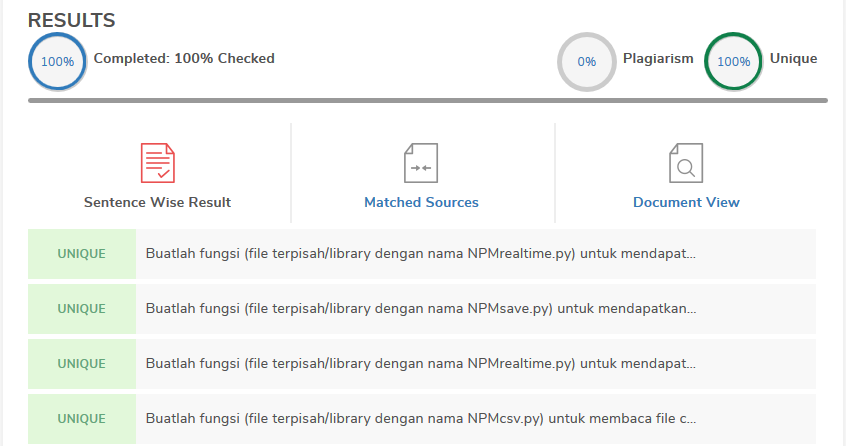
\includegraphics[width=10cm]{figures/5/1174077/praktek/cekpraktek.png}
	\centering
    \end{figure}
\end{enumerate}
\subsection{Ketrampilan Penanganan Error}
\begin{enumerate}
    \item Tuliskan  peringatan  error  yang  didapat  dari  mengerjakan  praktek ketiga  ini, dan  jelaskan  cara  penanganan  error  tersebut.   dan  Buatlah  satu fungsi  yang menggunakan try except untuk menanggulangi error tersebut.
\begin{itemize}
	\item Syntax Errors
	Syntax Errors adalah suatu keadaan saat kode python mengalami kesalahan penulisan. Solusinya adalah memperbaiki penulisan kode yang salah.
	
	\item Name Error
	NameError adalah exception yang terjadi saat kode melakukan eksekusi terhadap local name atau global name yang tidak terdefinisi. Solusinya adalah memastikan variabel atau function yang dipanggil ada atau tidak salah ketik.
	
	\item Type Error
	TypeError adalah exception yang akan terjadi apabila pada saat dilakukannya eksekusi terhadap suatu operasi atau fungsi dengan type object yang tidak sesuai. Solusi dari error ini adalah mengkoversi varibelnya sesuai dengan tipe data yang akan digunakan.
\end{itemize}
\par Fungsi yang menggunakan try except untuk menanggulangi error.
\lstinputlisting[firstline=1, 
lastline=16]{src/5/1174077/praktek/1174077.py}
\end{enumerate}
%%%%%%%%%%%%%%%%%%%%%%%%%%%%%%%%%%%%%%%%%%%%%%%%%%%%%%%%%%%%%%%%%%%%%%%%%%%%%%%%%%%%%%%%%%%%%%%%%%%%%%